\FloatBarrier
\subsection{Montículo 14}

\begin{figure}[!htbp]
    \centering
    % ----- Fila 1 -----
    \begin{subfigure}{0.48\textwidth}
        \centering
        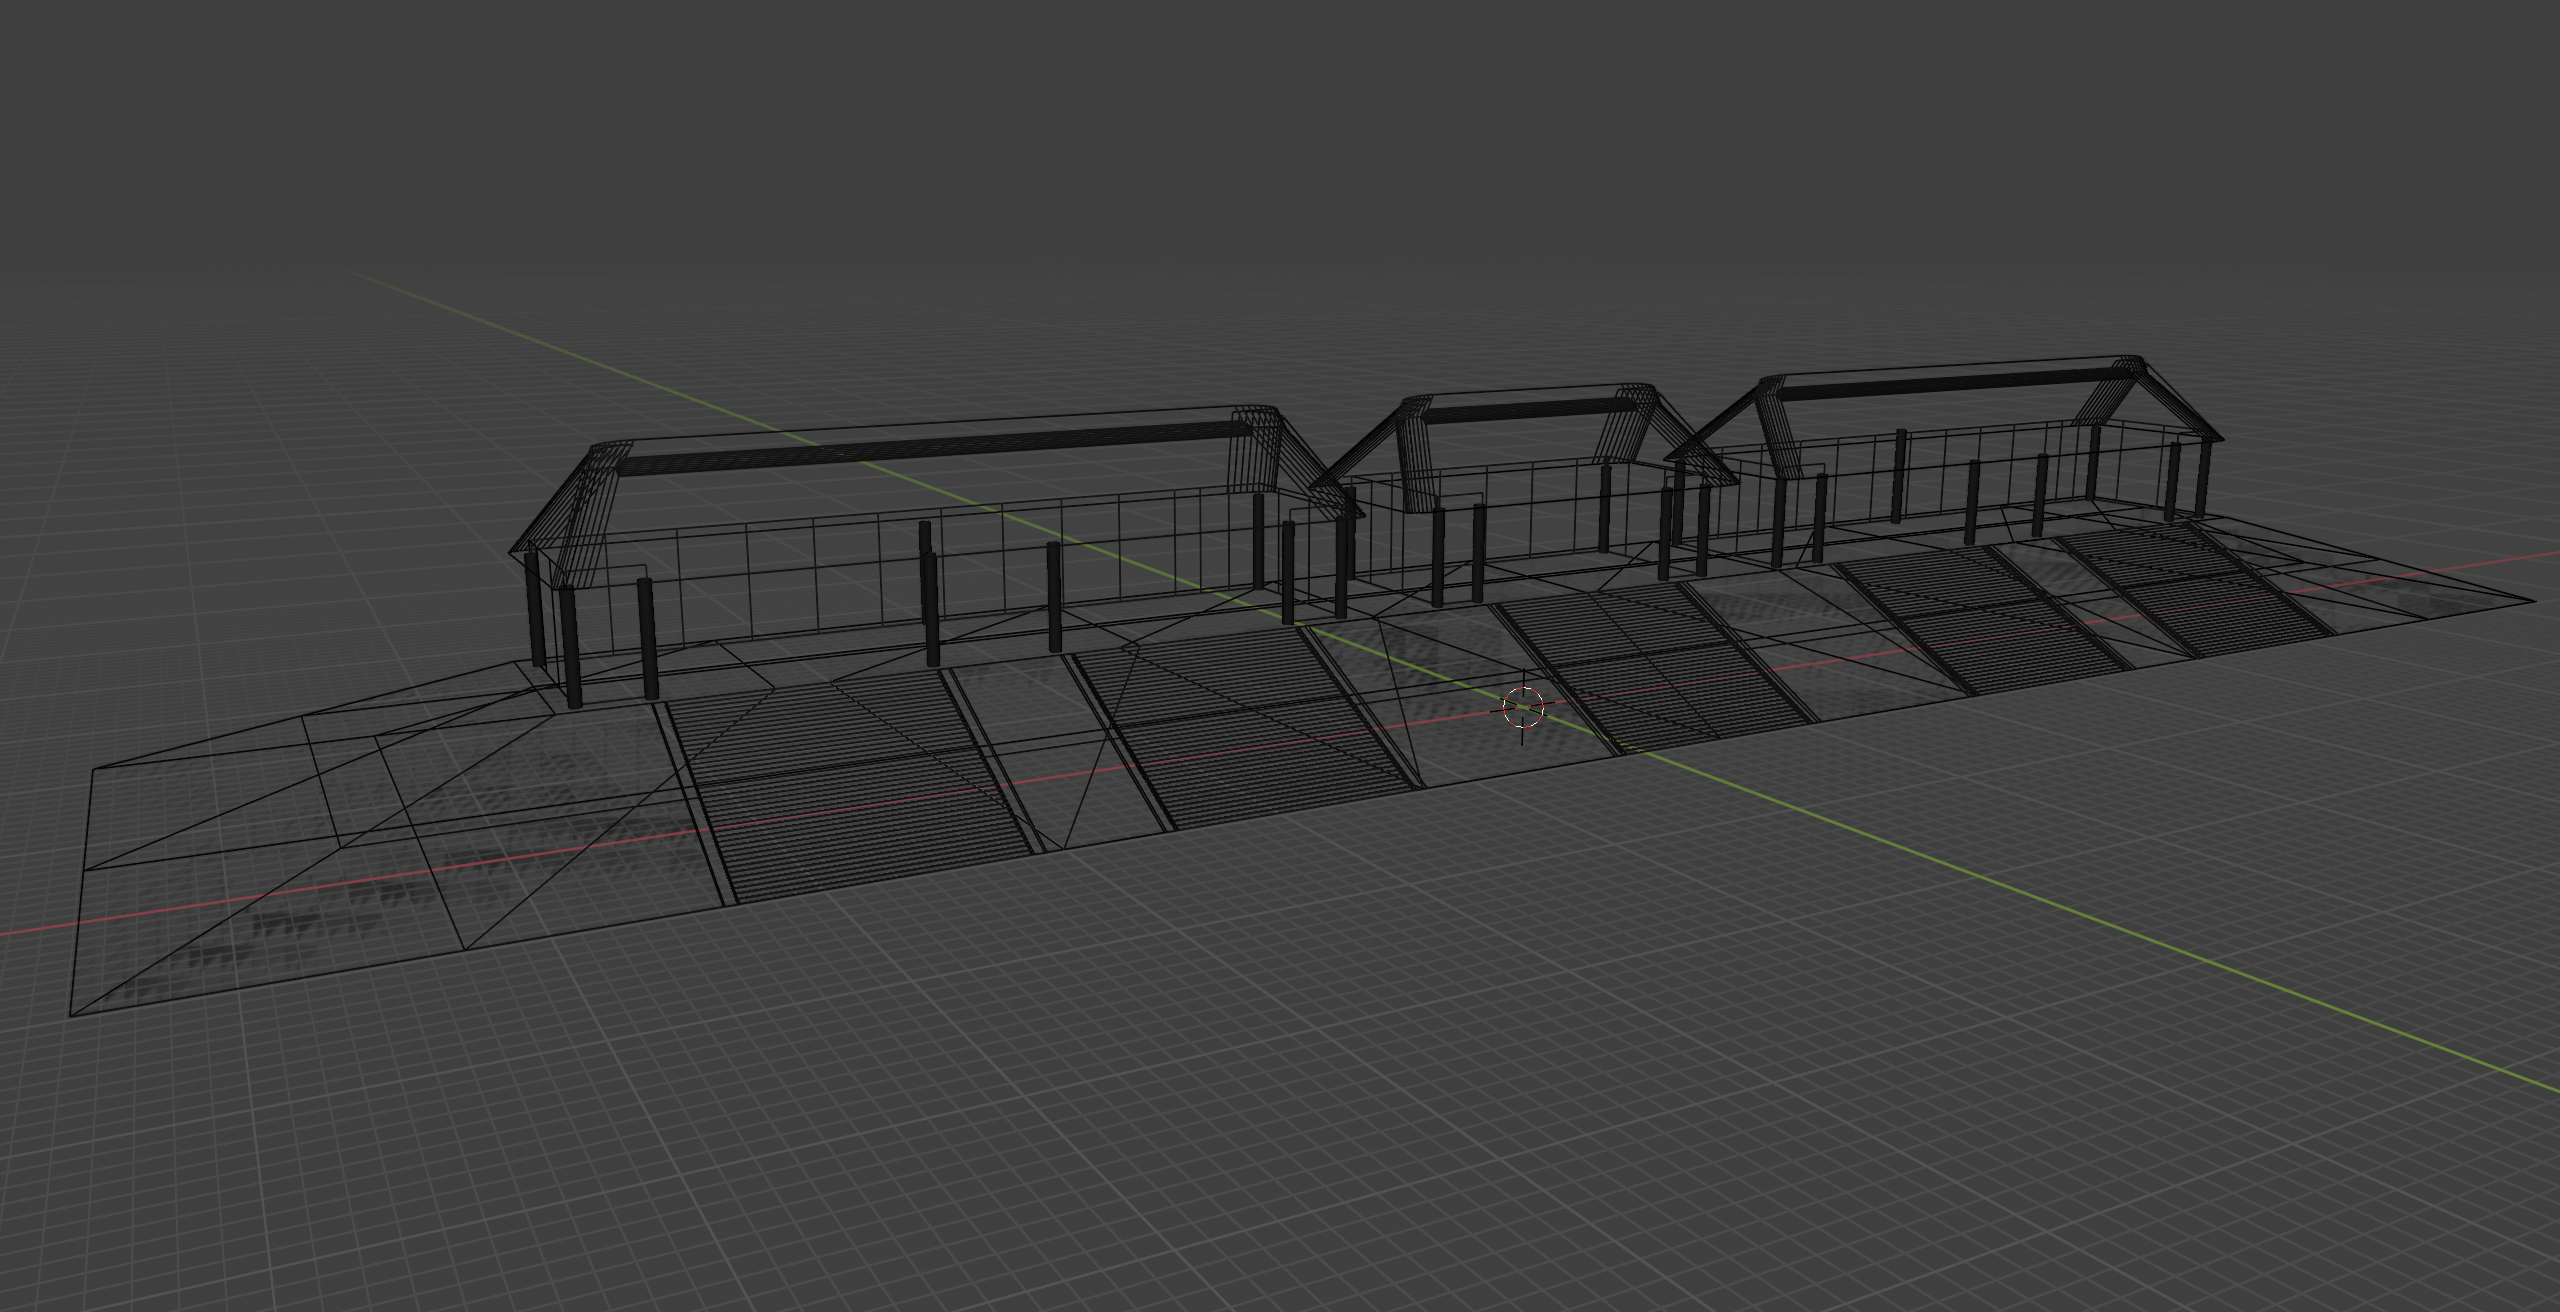
\includegraphics[width=0.85\linewidth]{resultados/figures/m14/m14_wireframe.png}
        \caption{Vista en malla (wireframe).}
        \label{fig:m14-wire}
    \end{subfigure}\hfill
    \begin{subfigure}{0.48\textwidth}
        \centering
        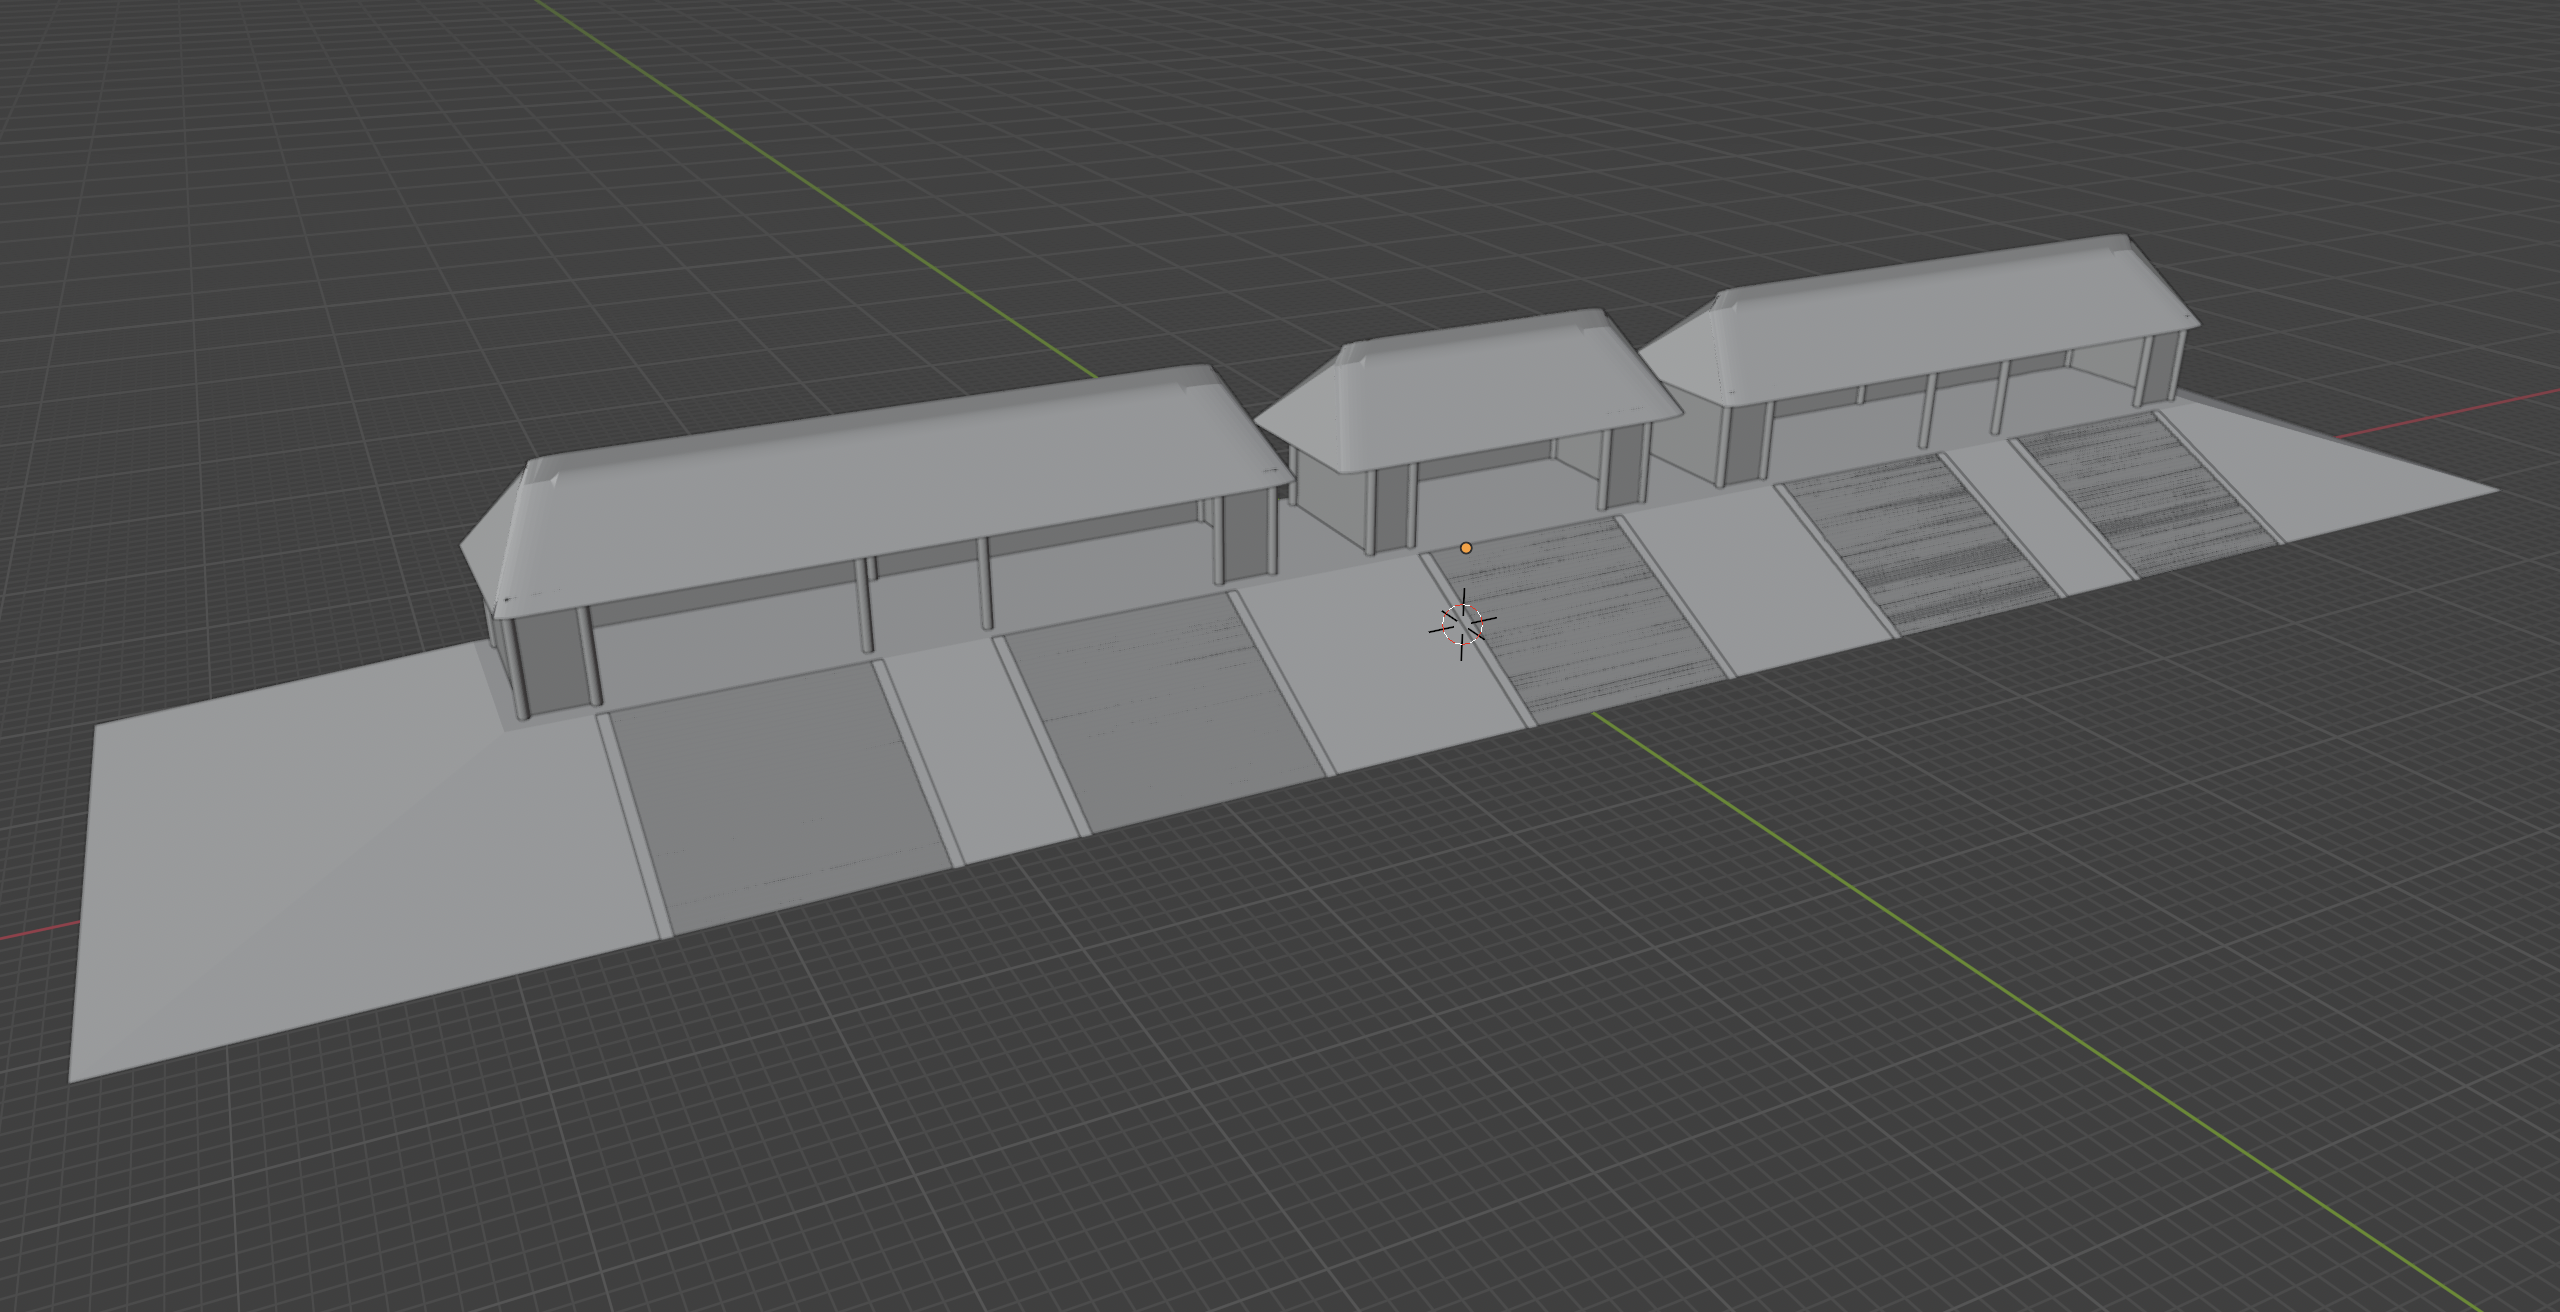
\includegraphics[width=0.85\linewidth]{resultados/figures/m14/m14_solid.png}
        \caption{Vista sólida sin texturas.}
        \label{fig:m14-solid}
    \end{subfigure}

    \vspace{0.5em}

    % ----- Fila 2 -----
    \begin{subfigure}{0.48\textwidth}
        \centering
        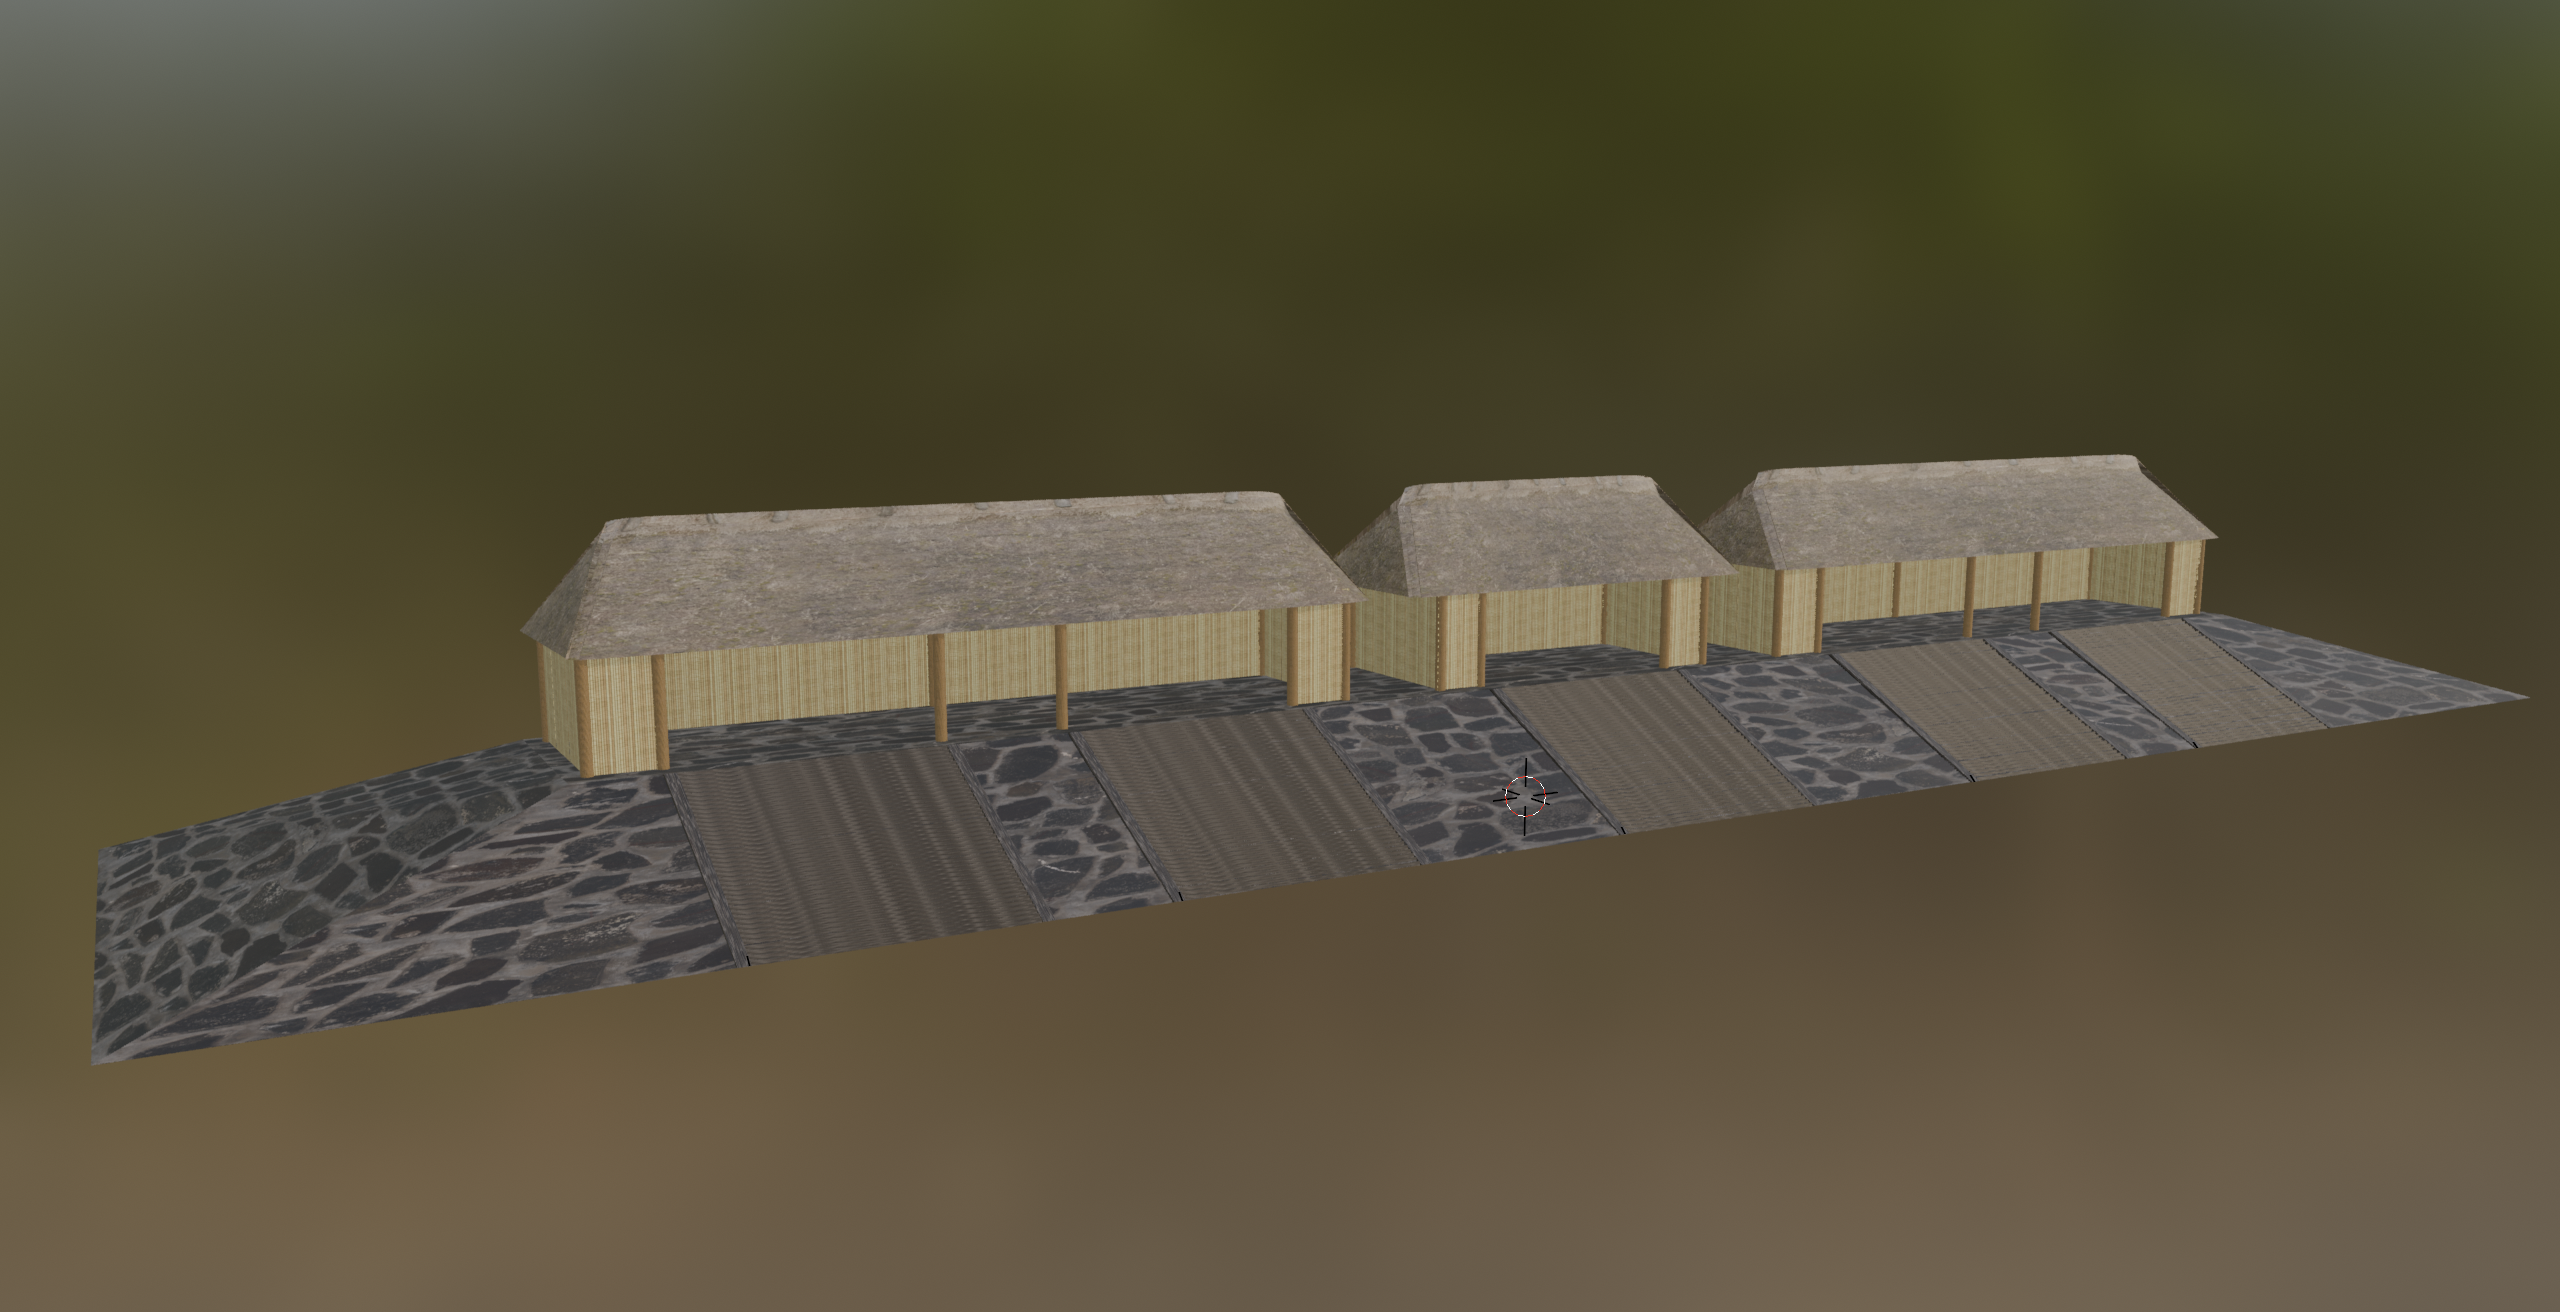
\includegraphics[width=0.85\linewidth]{resultados/figures/m14/m14_textured_viewport.png}
        \caption{Vista con materiales/texturas.}
        \label{fig:m14-textured}
    \end{subfigure}

    \caption{Montículo 14, panel de vistas.}
    \label{fig:m14-panel}
\end{figure}

\begin{figure}[!htbp]
    \centering
    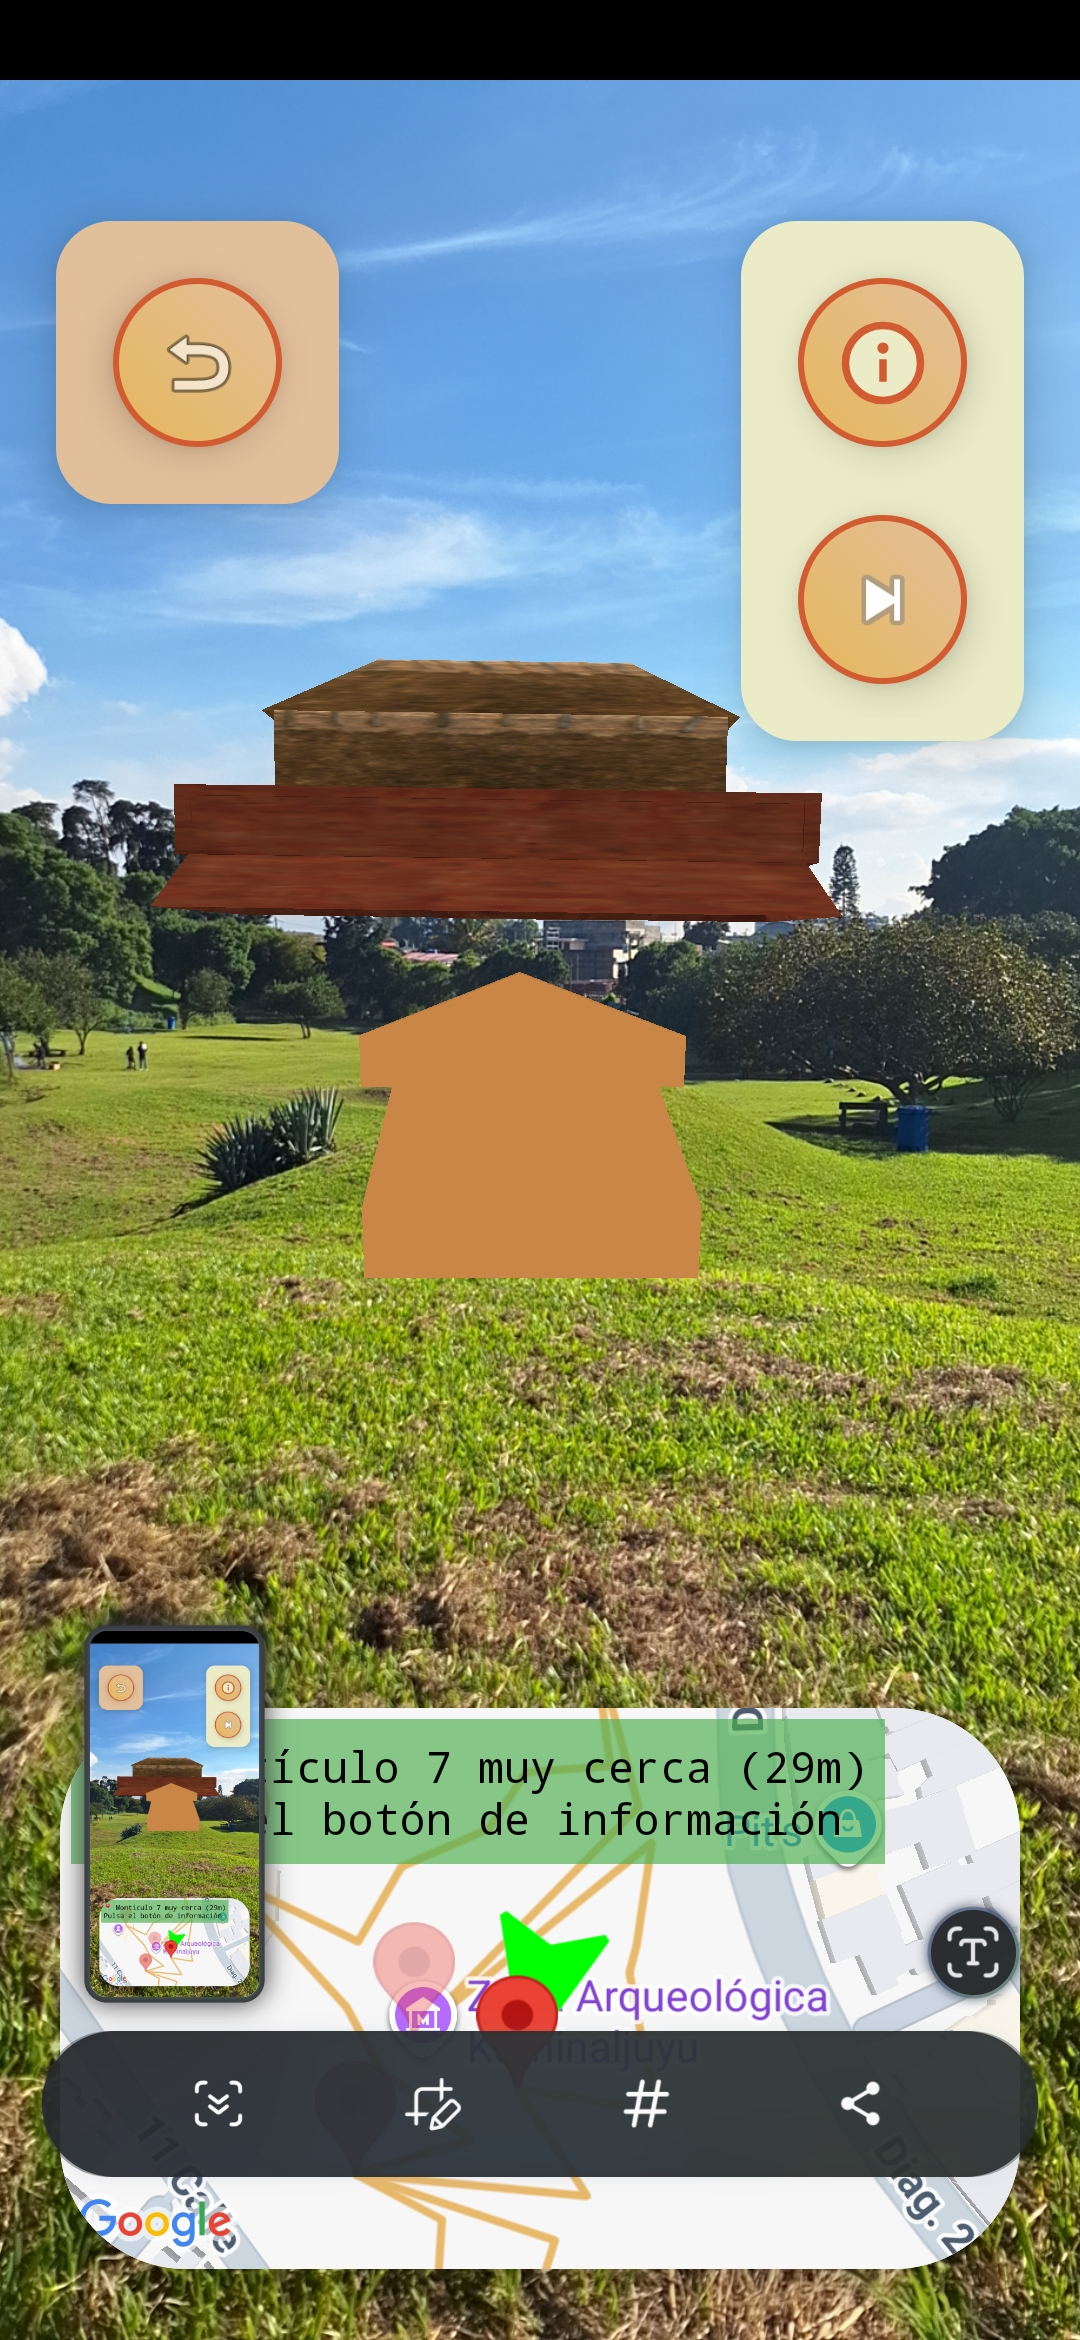
\includegraphics[width=0.28\linewidth]{resultados/figures/m3/m3_ar.jpg}
    \caption{Montículo 3 visualizado en la aplicación de realidad aumentada, mostrando la reconstrucción superpuesta en el entorno real del parque arqueológico.}
    \label{fig:m14-ar}
\end{figure}
\FloatBarrier
\clearpage